\chapter{Wstęp}

%---------------------------------------------------------------------------------------------
\section{Cel i zakres pracy}

Celem pracy jest implementacja metod fuzji sygnałów z akcelerometru, żyroskopu i magnetometru na potrzeby sterowania robotem balansującym oraz przygotowanie aplikacji do wizualizacji danych sensorycznych.

Fuzja sygnałów polegać będzie na zaimplementowaniu trzech wybranych algorytmów: filtra komplementarnego, filtra Kalmana oraz filtra Madgwicka. Wykorzystanie wszystkich trzech algorytmów, ma na celu uzyskanie informacji o kącie obrotu korpusu robota w poszczególnych osiach oraz sprawdzenie, czy z powodzeniem zastosować można je w algorytmie sterowania robota balansującego.

Aplikacja ma ułatwić implementację metod fuzji sygnałów dzięki przejrzystej formie prezentacji odczytów z czujników w postaci wykresów oraz trójwymiarowej wizualizacji orientacji robota. Dodatkową jej zaletą będzie możliwość komunikacji z robotem balansującym, w celu zadawania sterowania w postaci prędkości obrotowej silników, a także zmiana poszczególnych parametrów filtrów oraz regulatorów biorących udział w algorytmie sterowania robotem.

W celu przetestowania zaimplementowanych metod fuzji sygnałów pochodzących z czujników ruchu i algorytmu sterowania, wykonana zostanie konstrukcja dwukołowego robota balansującego. Wyposażona będzie w bezprzewodowy interfejs komunikacyjny, który ułatwi komunikację z aplikacją i usprawni etap testowania.

%---------------------------------------------------------------------------------------------
\section{Zadania do wykonania}

\begin{enumerate}
    \item Przegląd metod fuzji sygnałów
    \item Analiza ruchu robota balansującego oraz dostępnych czujników pod kątem zbierania danych dla sterownika ruchu 
    \item Implementacja akwizycji danych z czujników
    \item Opracowanie i implementacja fuzji sygnałów
    \item Przygotowanie aplikacji do wizualizacji zebranych i przetworzonych danych
    \item Budowa robota balansującego
    \item Testy symulacyjne i eksperymentalne
\end{enumerate}

%---------------------------------------------------------------------------------------------
\section{Przegląd gotowych konstrukcji}

Głównym problemem jaki pojawia się podczas budowy robota balansującego jest wyznaczenie kąta wychylenia od pionu jego korpusu. Jego dokładność i odporność na zakłócenia, znacząco wpływa na algorytm sterowania. Do najpopularniejszych rozwiązań tego problemu należy zastosowanie:
\begin{itemize}
    \item akcelerometru i żyroskopu
    \item enkodera 
    \item czujników odległości
\end{itemize}

Opisana w tej pracy konstrukcja pod względem wykorzystania danych pochodzących z akcelerometru i żyroskopu oraz zastosowania kaskady regulatorów PID w algorytmie sterowania, wzorowała się na konstrukcji robota ,,Kosmos'' opisanej w pracy \cite{Kosmos}.

\begin{figure}[h!]
    \centering
	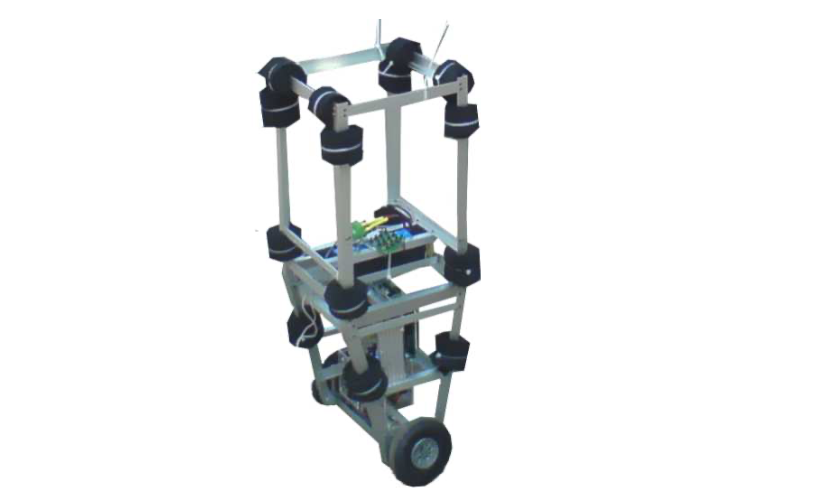
\includegraphics[width=0.5\textwidth]{Rysunki/Rozdzial01/Robot_Kosmos.png}
	\caption{Robot balansujący ,,Kosmos''}
\end{figure}

Innym dostępnym rozwiązaniem problemu balansowania w okolicach punktu równowagi robota balansującego jest robot balansujący wykorzystujący algorytm uczenia ze wzmocnieniem (Q-Learning), akcelerometr, żyroskop, oraz tym co różni go znacząco od poprzedniej konstrukcji, dodatkowo wspomaga się czujnikami odległości umieszczonymi w górnej części konstrukcji, na jej skrajnych brzegach \cite{Konstrukcja2}. Wychylenie robota obliczane na podstawie odczytów z czujników odległości odbywa się za pomocą funkcji trygonometrycznych. 

\begin{figure}[h!]
    \centering
	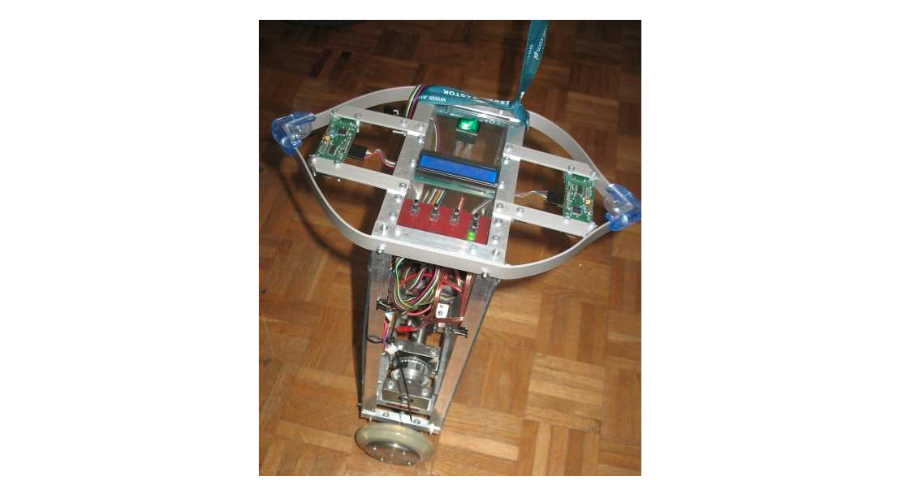
\includegraphics[width=0.5\textwidth]{Rysunki/Rozdzial01/Konstrukcja2.png}
	\caption{Robot balansujący wykorzystujący dodatkowe czujniki odległości}
\end{figure}

Czujnikiem jaki również można zastosować w tego typu konstrukcji, jest enkoder zamocowany na wale silnika. Daje on informację o kącie obrotu wału silnika, a informację tę wykorzystać można do wyznaczenia kąta wychylenia całej konstrukcji. Tego typu rozwiązanie zostało wykorzystane w pracy \cite{Konstrukcja3}.

\begin{figure}[h!]
    \centering
	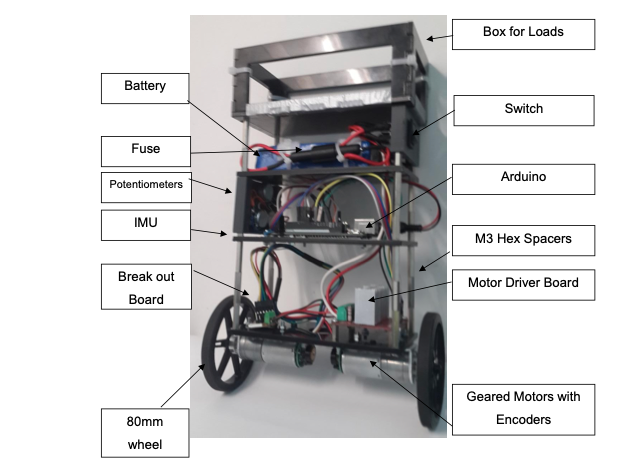
\includegraphics[width=0.5\textwidth]{Rysunki/Rozdzial01/Konstrukcja3.png}
	\caption{Robot balansujący wykorzystujący enkodery}
\end{figure}

Po dokonaniu przeglądu gotowych rozwiązań zdecydowano się na zastosowanie akcelerometru i żyroskopu do określenia kąta wychylenia robota, ze względu na chęć przetestowania metod fuzji sygnałów pochodzących z tych czujników oraz na zbyt niską dokładność kąta wychylenia wyznaczanego na podstawie czujników odległości czy enkodera. 

%---------------------------------------------------------------------------------------------
\section{Struktura pracy}

Drugi rozdział pracy zawiera wyprowadzenie równań dynamiki i opis algorytmu sterowania robota balansującego, na podstawie których wykonana została symulacja algorytmu sterowania. Kolejny rozdział pracy dotyczy wykorzystania danych pochodzących z akcelerometru, żyroskopu i magnetometru, w celu wyznaczenia kątów RPY. Mając do dyspozycji przetworzone dane z czujników w rozdziale czwartym opisano trzy algorytmy: filtr komplementarny, Kalmana, Madgwicka. Zostały one zaimplementowane i przetestowane na podstawie tego samego zestawu danych pochodzących z rzeczywistych czujników. Piąty i szósty rozdział to opis wykonania konstrukcji robota balansującego od strony elektronicznej, mechanicznej i oprogramowania oraz aplikacji do wizualizacji danych z niego pochodzących. Na sam koniec, w rozdziale siódmym podsumowano przeprowadzone na rzeczywistym robocie testy eksperymentalne, mające na celu porównanie przydatności tych trzech wymienionych wcześniej algorytmów na potrzeby sterowania robotem balansującym.